\begin{center}

  \begin{tabular}{rp{6cm}lp{12cm}}%{rl}

  % after \\: \hline or \cline{col1-col2} \cline{col3-col4} ...

  论文地址:& \href{https://arxiv.org/abs/2005.07115}{https://arxiv.org/abs/2005.07115} \\

  %源码:& \href{xxx}{xxx} \\

%  slides:& \href{http://yunshengb.com/wp-content/uploads/2017/03/nips_2018_r2l_workshop_talk.pdf}{{\footnotesize Convolutional Set Matching for Graph Similarity}}\\

  关键词:& \textbf{Graph Similarity, GNN} \\

  写于:& \date{2020-10-18}

  \end{tabular}

\end{center}

该论文\cite{xu2020hierarchical}着眼于大规模图的相似性计算问题。生物/化学中分子识别的时先将分子映射到分子组再在分子组的基础上计算分子的相似性,受到这个启发,论文提出了对大规模图的相似性计算方法 --- COSIM-GNN(Coarsen based Similarity Computation via Graph Neural Network),按照“embedding-coarsening-matching”的过程计算图的相似性。

\begin{figure}[h]
	\centering
	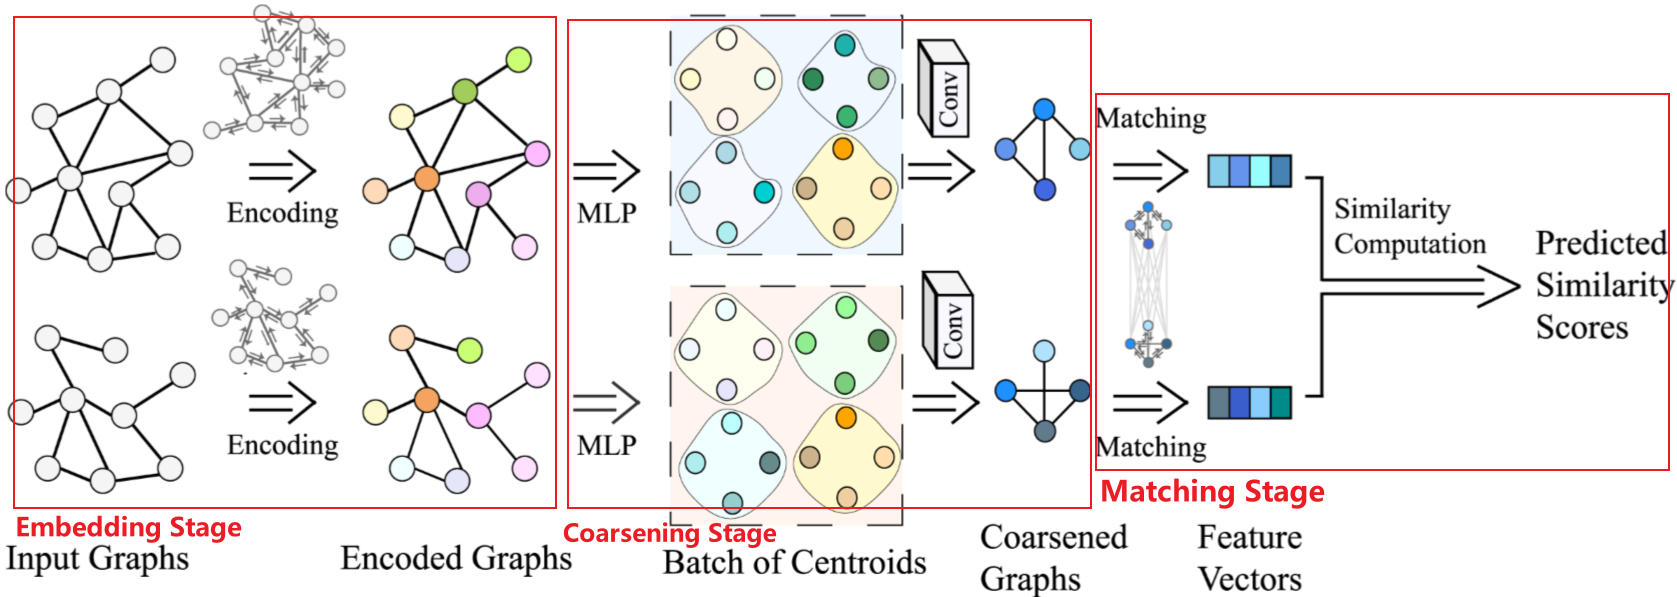
\includegraphics[width=.8\textwidth]{pics/COSIM.PNG}
	\caption{Overview of COSIM-GNN}
	\label{fig:cosim}
\end{figure}

\paragraph{COSIM-GNN思路}整体过程如图Fig.\ref{fig:cosim}所示,可以分为3个阶段:
\subparagraph{Embedding}对输入的两个图,使用GNN分别得到两个图的表征。

\subparagraph{Coarsening}对于Embedding阶段得到的图结点表征,Coarsening阶段,通过池化的方法得到一个粗化后的图。为了使得粗化后的图是和输入数据相关且是节点排列无关的,论文还提出了一个新的池化方法:Adaptive Pooling。该pooling方法在第一阶段的结点表征的基础上得到h个bathch --- 每个batch表示一个不同的图,基于这些batch来获得最终压缩后的图。\tred{为什么要获得h个batch呢?} --- 为了尽量使得到的反映原图的压缩图。具体细节可参看论文(这一部分我没看太懂)。

\subparagraph{Matching}之前的两个阶段中,是分别在输入的两个图上执行这两个阶段。每个图的结果,都只使用了图本身的信息,Matching阶段则涉及到两个图之间的交互,在两个图的基础上一起计算相似性。具体可以使用一些匹配的方法来计算得到它们的相似性,如GSimCNN


\paragraph{方法解决的问题/优势}
\begin{itemize}
	\item 针对大图的相似性计算给出了解决方法
	\item 利用了图之间的信息计算图的相似性,并且通过coarsening降低了这一过程的计算开销
	%\item 

\end{itemize}

\paragraph{方法的局限性/未来方向}
\begin{itemize}
	\item 改进粗化图的方法
	\item 改进图匹配的方法
\end{itemize}
